\documentclass[notes,11pt, aspectratio=169]{beamer}

\usepackage{pgfpages}
% These slides also contain speaker notes. You can print just the slides,
% just the notes, or both, depending on the setting below. Comment out the want
% you want.
\setbeameroption{hide notes} % Only slide
%\setbeameroption{show only notes} % Only notes
%\setbeameroption{show notes on second screen=right} % Both

\usepackage{helvet}
\usepackage[default]{lato}
\usepackage{array}
\usepackage{tgbonum}

\usepackage{tikz}
\usepackage{verbatim}
\setbeamertemplate{note page}{\pagecolor{yellow!5}\insertnote}
\usetikzlibrary{positioning}
\usetikzlibrary{snakes}
\usetikzlibrary{calc}
\usetikzlibrary{arrows}
\usetikzlibrary{decorations.markings}
\usetikzlibrary{shapes.misc}
\usetikzlibrary{matrix,shapes,arrows,fit,tikzmark}
\usepackage{amsmath}
\usepackage{mathpazo}
\usepackage{hyperref}
\usepackage{lipsum}
\usepackage{multimedia}
\usepackage{graphicx}
\usepackage{multirow}
\usepackage{graphicx}
\usepackage{dcolumn}
\usepackage{bbm}
\newcolumntype{d}[0]{D{.}{.}{5}}

\usepackage{changepage}
\usepackage{appendixnumberbeamer}
\newcommand{\beginbackup}{
   \newcounter{framenumbervorappendix}
   \setcounter{framenumbervorappendix}{\value{framenumber}}
   \setbeamertemplate{footline}
   {
     \leavevmode%
     \hline
     box{%
       \begin{beamercolorbox}[wd=\paperwidth,ht=2.25ex,dp=1ex,right]{footlinecolor}%
%         \insertframenumber  \hspace*{2ex} 
       \end{beamercolorbox}}%
     \vskip0pt%
   }
 }
\newcommand{\backupend}{
   \addtocounter{framenumbervorappendix}{-\value{framenumber}}
   \addtocounter{framenumber}{\value{framenumbervorappendix}} 
}


\usepackage{graphicx}
\usepackage[space]{grffile}
\usepackage{booktabs}
\newcommand\independent{\protect\mathpalette{\protect\independenT}{\perp}}
\def\independenT#1#2{\mathrel{\rlap{$#1#2$}\mkern2mu{#1#2}}}
\DeclareMathOperator{\Supp}{Supp}

% These are my colors -- there are many like them, but these ones are mine.
\definecolor{blue}{RGB}{0,114,178}
\definecolor{red}{RGB}{213,94,0}
\definecolor{yellow}{RGB}{240,228,66}
\definecolor{green}{RGB}{0,158,115}

\hypersetup{
  colorlinks=false,
  linkbordercolor = {white},
  linkcolor = {blue}
}


%% I use a beige off white for my background
\definecolor{MyBackground}{RGB}{255,253,218}

%% Uncomment this if you want to change the background color to something else
%\setbeamercolor{background canvas}{bg=MyBackground}

%% Change the bg color to adjust your transition slide background color!
\newenvironment{transitionframe}{
  \setbeamercolor{background canvas}{bg=yellow}
  \begin{frame}}{
    \end{frame}
}

\setbeamercolor{frametitle}{fg=blue}
\setbeamercolor{title}{fg=black}
\setbeamertemplate{footline}[frame number]
\setbeamertemplate{navigation symbols}{} 
\setbeamertemplate{itemize items}{-}
\setbeamercolor{itemize item}{fg=blue}
\setbeamercolor{itemize subitem}{fg=blue}
\setbeamercolor{enumerate item}{fg=blue}
\setbeamercolor{enumerate subitem}{fg=blue}
\setbeamercolor{button}{bg=MyBackground,fg=blue,}



% If you like road maps, rather than having clutter at the top, have a roadmap show up at the end of each section 
% (and after your introduction)
% Uncomment this is if you want the roadmap!
% \AtBeginSection[]
% {
%    \begin{frame}
%        \frametitle{Roadmap of Talk}
%        \tableofcontents[currentsection]
%    \end{frame}
% }
\setbeamercolor{section in toc}{fg=blue}
\setbeamercolor{subsection in toc}{fg=red}
\setbeamersize{text margin left=1em,text margin right=1em} 

\newenvironment{wideitemize}{\itemize\addtolength{\itemsep}{10pt}}{\enditemize}

\usepackage{environ}
\NewEnviron{videoframe}[1]{
  \begin{frame}
    \vspace{-8pt}
    \begin{columns}[onlytextwidth, T] % align columns
      \begin{column}{.70\textwidth}
        \begin{minipage}[t][\textheight][t]
          {\dimexpr\textwidth}
          \vspace{8pt}
          \hspace{4pt} {\Large \sc \textcolor{blue}{#1}}
          \vspace{8pt}
          
          \BODY
        \end{minipage}
      \end{column}%
      \hfill%
      \begin{column}{.38\textwidth}
        \colorbox{green!20}{\begin{minipage}[t][1.2\textheight][t]
            {\dimexpr\textwidth}
            Face goes here
          \end{minipage}}
      \end{column}%
    \end{columns}
  \end{frame}
}

\title[]{\textcolor{blue}{Propensity Scores}}
\author[PGP]{}
\institute[FRBNY]{\small{Paul Goldsmith-Pinkham}}
\date{\today}


\begin{document}

%%% TIKZ STUFF
\tikzset{   
        every picture/.style={remember picture,baseline},
        every node/.style={anchor=base,align=center,outer sep=1.5pt},
        every path/.style={thick},
        }
\newcommand\marktopleft[1]{%
    \tikz[overlay,remember picture] 
        \node (marker-#1-a) at (-.3em,.3em) {};%
}
\newcommand\markbottomright[2]{%
    \tikz[overlay,remember picture] 
        \node (marker-#1-b) at (0em,0em) {};%
}
\tikzstyle{every picture}+=[remember picture] 
\tikzstyle{mybox} =[draw=black, very thick, rectangle, inner sep=10pt, inner ysep=20pt]
\tikzstyle{fancytitle} =[draw=black,fill=red, text=white]
%%%% END TIKZ STUFF

% Title Slide
\begin{frame}
\maketitle

\end{frame}

\begin{frame}{This week}
 
  \begin{wideitemize}
  \item  Discuss two points: propensity scores and interference
    \begin{enumerate}
    \item Propensity scores
    \item Interference and violations of SUTVA
    \end{enumerate}
  \item For today, propensity scores. The end goal: 
    \begin{itemize}
    \item Have a framework for discussing subpopulations
      being treated
    \item A way to link to an underlying economic model
    \end{itemize}
  \item This will provide structure for us later
  \end{wideitemize}
\end{frame}


% INTRO
\begin{frame}{Estimation of treatment effects}
\begin{columns}[T] % align columns
\begin{column}{.65\textwidth}
  \begin{wideitemize}
  \item Recall two results:
    \begin{itemize}
    \item \underline{Horvitz-Thompson Estimator}
      \begin{equation*}
        \hat{\bar{\tau}}_{HT} = n^{-1}\sum_{i}\pi^{-1}_{i}Y_{i}D_{i} - (1-\pi_{i})^{-1}Y_{i}(1-D_{i})
      \end{equation*}
      Unbiased estimator of $\tau_{ATE}$ , here $\pi_{i} = Pr(D_{i} = 1 | X_{i})$
    \item \underline{Conditional strong ignorability}: $D_{i}$ is \emph{strongly
        ignorable} conditional on a vector $\mathbf{X}_{i}$ if
    \begin{enumerate}
    \item $(Y_{i}(0), Y_{i}(1)) \independent D_{i} | \mathbf{X}_{i} $
    \item $\exists \epsilon > 0$ s.t. $\epsilon < \Pr(D_{i} = 1 | X_{i}) < 1-\epsilon_{i}$
    \end{enumerate}
  \end{itemize}
\item Key: $\pi(X_{i}) = Pr(D_{i} = 1 | X_{i})$ is important
  \begin{itemize}
  \item This is the \emph{propensity score}.
  \item We will dive into this today
  \end{itemize}
  \end{wideitemize}
\end{column}%
\hfill%
\begin{column}{.4\textwidth}

\end{column}%
\end{columns}
\end{frame}

% INTRO
\begin{frame}{Why does the propensity score matter? Rosenbaum-Rubin (1983)}
\begin{columns}[T] % align columns
\begin{column}{.75\textwidth}
  \begin{wideitemize}
  \item Note our strong ignorability condition,
    $(Y_{i}(0), Y_{i}(1)) \independent D_{i} | \mathbf{X}_{i}$
    conditions on $\mathbf{X}_{i}$, which can be quite high
    dimensional
  \item Key result from Rosenbaum-Rubin: if the above holds, then so does
    $(Y_{i}(0), Y_{i}(1)) \independent D_{i} | \pi(\mathbf{X}_{i})$.
    \begin{itemize}
    \item The intuition comes from the fact that conditional on $\pi(\mathbf{X}_{i})$, the distribution of $X$ is the same for the treated and untreated, and thus $X_{i}$ and $D_{i}$ are independent.
    \end{itemize}
  \item Why does this matter? Crucially, solves a high-dimensional
    problem -- now we just need to condition on a single scalar value
    ($\pi_{i}$)
    \end{wideitemize}
\end{column}%
\hfill%
\begin{column}{.4\textwidth}

\end{column}%
\end{columns}
\end{frame}


\begin{frame}{Layering complications -- how to match?}
\begin{columns}[T] % align columns
\begin{column}{.55\textwidth}
  \begin{wideitemize}
  \item<1-> You ideally match on exactly the propensity score
    \begin{itemize}
    \item However, ``Unfortunately, exact matches even on a scalar balancing score are often impossible to obtain, so methods which seek approximate matches must be used.''
    \item This creates bias. How? Consider this example from Aronow and Miller
    \end{itemize}
  \item<2-> We need to construct $E(Y_{i}(1) | \pi(X)) $ and
    $E(Y_{i}(0) 1) | \pi(X))$ for each observation. How do we pick now?
    Closest p-value? What are the issues with this?
    \begin{itemize}
    \item We picked unit $i = 2$ for unit 1, but unit $4$ was very
      close. Why not pick that one?
    \item More generally, this approach has challenges for inference,
      especially with $\pi(\mathbf{X})$ unknown (see Abadie and Imbens
      (2008))
    \end{itemize}
  \end{wideitemize}
\end{column}%
\hfill%
\begin{column}{.5\textwidth}
  \small
  \only<1>{
  \begin{tabular}{ccccccc}
    $i$ & $Y_{i}(0)$ & $Y_{i}(1)$ & $D_{i}$ & $X_{i1}$ & $X_{i2}$ & $\pi(\mathbf{X}_{i})$\\
    \midrule
    1 & - & 2 & 1 & 1 & 7 & 0.33\\
    2 & 5 & - & 0 & 0 & 7 & 0.14\\    
    3 & - & 3 & 1 & 10 & 3 & 0.73\\
    4 & - & 10 & 1 & 3 & 1 & 0.35\\
    5 & - & 2 & 1 & 5 & 2 & 0.78\\
    6 & 0 & - & 0 & 7 & 0 & 0.70\\        
  \end{tabular}
}
  \only<2>{
  \begin{tabular}{ccccccc}
    $i$ & $Y_{i}(0)$ & $Y_{i}(1)$ & $D_{i}$ & $X_{i1}$ & $X_{i2}$ & $\pi(\mathbf{X}_{i})$\\
    \midrule
    1 & \textcolor{red}{5} & 2 & 1 & 1 & 7 & 0.33\\
    2 & 5 & \textcolor{red}{2} & 0 & 0 & 7 & 0.14\\    
    3 & \textcolor{red}{0} & 3 & 1 & 10 & 3 & 0.73\\
    4 & \textcolor{red}{5} & 10 & 1 & 3 & 1 & 0.35\\
    5 & \textcolor{red}{0} & 2 & 1 & 5 & 2 & 0.78\\
    6 & 0 & \textcolor{red}{3} & 0 & 7 & 0 & 0.70\\        
  \end{tabular}
  }
\end{column}%
\end{columns}
\end{frame}

\begin{frame}{What to do instead of matching? }
\begin{columns}[T] % align columns
\begin{column}{.8\textwidth}
  \begin{wideitemize}
  \item Note that matching addresses the problem literally
    \begin{itemize}
    \item Since the ignorability statement is with respect to $X$, natural to match on it
    \item But this ignores the estimand -- always focus on the estimand!
    \end{itemize}
  \item Key result: consider the follow result about the population
    version of the Horvitz-Thompson estimator, sometimes referred to
    as the inverse probability weighting estimator:
    \begin{equation*}
      E(\tau_{i}) = E\left(\underbrace{\frac{Y_{i}D_{i}}{\pi(\mathbf{X})}}_{E(Y_{i}(1))} - \underbrace{\frac{Y_{i}(1-D_{i})}{1-\pi(\mathbf{X})}}_{E(Y_{i}(0))}\right)
    \end{equation*}
  \item This is an amazing result!
    \begin{itemize}
    \item Under discrete $\mathbf{X}$, this collapses to what we would logically do anyway
    \end{itemize}
    \end{wideitemize}
\end{column}%
\hfill%
\begin{column}{.4\textwidth}

\end{column}%
\end{columns}
\end{frame}

\begin{frame}{A more stable IPW estimator}
\begin{columns}[T] % align columns
\begin{column}{.8\textwidth}
  \begin{wideitemize}
  \item The IPW approach works well, but in small samples can be high
    variance if you get big $\pi(\mathbf{X})$ values.
    \begin{itemize}
    \item     We can slightly improve on it using the stabilized IPW estimator:
      \begin{equation*}
        \hat{\tau}_{SIPW} = \frac{\frac{1}{n}\sum_{i}\frac{Y_{i}D_{i}}{\hat{\pi}(\mathbf{X}_{i})}}{\frac{1}{n}\sum_{i}\frac{D_{i}}{\hat{\pi}(\mathbf{X}_{i})}} - \frac{\frac{1}{n}\sum_{i}\frac{Y_{i}(1-D_{i})}{1-\hat{\pi}(\mathbf{X})}}{\frac{1}{n}\sum_{i}\frac{(1-D_{i})}{1-\hat{\pi}(\mathbf{X})}}
      \end{equation*}
    \end{itemize}
  \item This estimator benefits by adjusting for unusually high or low
    values of $\pi(\mathbf{X})$
    \begin{itemize}
    \item Note that this estimator effectively constructs $w_{i} = \frac{\frac{D_{i}}{\hat{\pi}(\mathbf{X}_{i})}}{\frac{1}{n}\sum_{i}\frac{D_{i}}{\hat{\pi}(\mathbf{X}_{i})}} $ for the treated group -- reweighting by the average density within the sample
    \item In the limit, this just goes to one but works well in finite samples
    \end{itemize}
    \end{wideitemize}
\end{column}%
\hfill%
\begin{column}{.4\textwidth}

\end{column}%
\end{columns}
\end{frame}

\begin{frame}{True vs. estimated propensity scores?}
\begin{columns}[T] % align columns
\begin{column}{.9\textwidth}
  \begin{wideitemize}
  \item True propensity scores are only known sometimes (e.g. randomized experiments)
  \item In most non-experimental settings, the p-score is unknown and must be estimated
  \item When estimating, we have two cases:
    \begin{itemize}
    \item If $X$ is discrete, we know that $\hat{\pi}(X)$ can be an exact approximation (why?)
    \item If $X$ is \emph{not} discrete (or high-dimensional), how should we approximate it?
    \end{itemize}
  \item We need to estimate $\pi(X)$ in a way that is flexible and
    will converge to the truth in the limit -- e.g. semi-parametric
    estimation of $\pi$
    \begin{itemize}
    \item Note a linear model of $\pi$ will inherently be wrong b/c probabilities are bounded between 0 and 1
    \item Practical implication: logit estimation of $\pi(X)$ is
      reasonable, allowing for flexible specification of $X$
      \begin{itemize}
      \item As dimension of $X$ grows, ML / lasso style models grow in
        value
      \end{itemize}
    \end{itemize}
    \end{wideitemize}
\end{column}%
\hfill%
\begin{column}{.4\textwidth}

\end{column}%
\end{columns}
\end{frame}

\begin{frame}{True vs. estimated propensity scores?}
\begin{columns}[T] % align columns
\begin{column}{.9\textwidth}
  \begin{wideitemize}
  \item Important result: \emph{even if you know the true function
      $\pi(\mathbf{X})$}, better to use the estimated function than
    the truth (Imbens, Hirano and Ridder (2002))
    \begin{itemize}
    \item Intuition: the deviations from the ``true'' propensity score
      ($\hat{\pi}(\mathbf{X}) - \pi(\mathbf{X})$) are informative for
      the estimation of the treatment effects (a la extra moment
      restrictions in GMM)
    \end{itemize}
  \item Clear tension -- as dimension of controls increases, the noisiness in $\pi$ grows as well
    \begin{itemize}
    \item Is it reasonable to consider this a good research design?
    \end{itemize}
    \item We will consider this in a basic way on the homework
    \end{wideitemize}
\end{column}%
\hfill%
\begin{column}{.4\textwidth}

\end{column}%
\end{columns}
\end{frame}


\begin{frame}{Contrasting propensity scores with regression}
\begin{columns}[T] % align columns
\begin{column}{.8\textwidth}
  \begin{wideitemize}
  \item Say we have strong ignorability and we run the following regression
    \begin{equation*}
      Y_{i} = \gamma_{0} + D_{i}\tau + X_{i1}\gamma_{1} + X_{i2}\gamma_{2} + u_{i}
    \end{equation*}
    How should we contrast this to some pscore approach?
    \pause
  \item Revisit the Aronow and Miller example
    \end{wideitemize}
  \begin{tabular}{ccccccc}
    $i$ & $Y_{i}(0)$ & $Y_{i}(1)$ & $D_{i}$ & $X_{i1}$ & $X_{i2}$ & $\pi(\mathbf{X}_{i})$\\
    \midrule
    1 & $\hat{\gamma}_{0} + \hat{\tau} \cdot D_{i} + \hat{\gamma}_{1} \cdot X_{i1} + \hat{\gamma}_{2} \cdot X_{i2}$  & 2 & 1 & 1 & 7 & 0.33\\
    2 & 5 & $\hat{\gamma}_{0} + \hat{\tau} \cdot D_{i} + \hat{\gamma}_{1} \cdot X_{i1} + \hat{\gamma}_{2} \cdot X_{i2}$ & 0 & 0 & 7 & 0.14\\    
    3 & $\hat{\gamma}_{0} + \hat{\tau} \cdot D_{i} + \hat{\gamma}_{1} \cdot X_{i1} + \hat{\gamma}_{2} \cdot X_{i2}$ & 3 & 1 & 10 & 3 & 0.73\\
    4 & $\hat{\gamma}_{0} + \hat{\tau} \cdot D_{i} + \hat{\gamma}_{1} \cdot X_{i1} + \hat{\gamma}_{2} \cdot X_{i2}$ & 10 & 1 & 3 & 1 & 0.35\\
    5 & $\hat{\gamma}_{0} + \hat{\tau} \cdot D_{i} + \hat{\gamma}_{1} \cdot X_{i1} + \hat{\gamma}_{2} \cdot X_{i2}$ & 2 & 1 & 5 & 2 & 0.78\\
    6 & 0 & $\hat{\gamma}_{0} + \hat{\tau} \cdot D_{i} + \hat{\gamma}_{1} \cdot X_{i1} + \hat{\gamma}_{2} \cdot X_{i2}$ & 0 & 7 & 0 & 0.70\\        
  \end{tabular}
\end{column}%
\hfill%
\begin{column}{.4\textwidth}

\end{column}%
\end{columns}
\end{frame}


\begin{frame}{Contrasting propensity scores with regression}
\begin{columns}[T] % align columns
\begin{column}{.8\textwidth}

  \begin{wideitemize}
  \item When will this approach do well?
    \begin{itemize}
    \item If the outcome conditional expectation function is approximately linear
    \item We don't have to extrapolate too much across the support of $\mathbf{X}_{i}$
    \item Put differently -- OLS is the best linear predictor. We might as well take advantage of that fact!
    \end{itemize}
  \item Key point: this is just another way to infer the missing
    data. We will rely on regression heavily, but important to not
    forget that this is just another way to infer values of missing
    data.
  \item Substantial \emph{empirical} debate about which approach is best.
    \begin{itemize}
    \item Debatable in finite samples but Imbens Hirano \& Ridder
      (2003) shows that if pscore is unknown, using the estimated
      non-parametric pscore is semiparametric efficient
    \item We will revisit in linear regression
    \end{itemize}
  \end{wideitemize}
\end{column}%
\hfill%
\begin{column}{.4\textwidth}

\end{column}%
\end{columns}
\end{frame}


\begin{frame}{Angrist and Pischke's advocation for regression}
\begin{columns}[T] % align columns
  \begin{column}{.65\textwidth}
    \begin{quote}
      We believe regression should be the starting point for most empirical projects. This is not a theorem; undoubtedly, there are circumstances where propensity score matching provides more reliable estimates of average causal effects. The first reason we don't find ourselves on the propensity-score bandwagon is practical: there are many details to be filled in when implementing propensity-score matching - such as how to model the score and how to do inference - these details are not yet standardized. Different researchers might therefore reach very different conclusions, even when using the same data and covariates. Moreover, as we've seen with the Horvitz-Thompson estimands,there isn't very much theoretical daylight between regression and propensity-score weighting.
      \end{quote}
\end{column}%
\hfill%
\begin{column}{.35\textwidth}
\includegraphics[width=\linewidth]{images/mhe.jpg}
\end{column}%
\end{columns}
\end{frame}


\begin{frame}{Angrist and Pischke's advocation for regression}
\begin{columns}[T] % align columns
  \begin{column}{.65\textwidth}
    \begin{wideitemize}
    \item This point about the IPW estimator comes from the fact that
      when the covariates are discrete, a fully saturated regression
      model can be written as an IPW estimator.
    \item See MHE for this discussion, but the intuition comes from a
      correctly specified propensity score (due to the full
      saturation) and residual regression.
    \item The punchline is that when we start having to worry about
      the pscore (i.e. in worlds with many covariates and/or
      continuous covariates), life gets complicated.
    \item As we will discuss below, forces us to think about overlap of covariates and balance
      \begin{itemize}
      \item E.g. comparability between treated and untreated groups
      \end{itemize}
    \end{wideitemize}
\end{column}%
\hfill%
\begin{column}{.35\textwidth}
\includegraphics[width=\linewidth]{images/mhe.jpg}
\end{column}%
\end{columns}
\end{frame}

\begin{frame}{Crucial empirical context: Lalonde (1986), Dehijia and Wahba (1999,2002), Smith and Todd (2005)}
  \begin{wideitemize}
    \item There was a randomized intervention called the NSW (National Supported Work Demonstration) -- temporary employment program to give work experience
    \item Key takeaway from Lalonde (1986) -- non-experimental
      analaysis of this program (e.g. defining control gorup using
      non-experimental data) would have given biased estimates compared to experimental approach
      \begin{itemize}
      \item That's bad! ``This comparison shows that many of the econometric proce-
 dures do not replicate the experimentally determined results.''
      \end{itemize}
    \item Dehijia and Wahba reanalyze this data using pscore methods
      \begin{itemize}
      \item Key point -- using pscores gets you closer \emph{and}
        provides a form of diagnostics on how comparable the groups
      \item Necessary consequence of these methods -- need to
        subsample the data to have 2 years of pre-treatment data to
        match well
      \end{itemize}
    \item Smith and Todd reanalyze this approach, and argue that the
      \emph{subsampling} predisposes to a group where the analysis is ``easy.''
      \begin{itemize}
      \item Dehijia's response -- ``of course!''
      \end{itemize}
      
  \end{wideitemize}
  
\end{frame}

\begin{frame}{Dehijia's conclusion}
\includegraphics[width=0.7\linewidth]{images/dehijia1.png}
\end{frame}


\begin{frame}{The problem with propensity scores/matching/observational data}
\begin{columns}[T] % align columns
\begin{column}{.7\textwidth}
  \begin{wideitemize}
  \item We initially motivated strong ignorablity under settings with
    random assignment or something approximating it
    \begin{itemize}
    \item However, in many settings, researchers will use exclusively
      observational data and use this to estimate a causal effect
    \end{itemize}
  \item To quote Heckman, Todd and Ichimura: ``Ironically, missing data give rise to the problem of causal inference, but missing data, i.e. the unobservables producing variation in D conditional on X, are also required to solve the problem of causal inference.''
  \item In other words -- if we're controlling for $X$, there must be additional source of variation in $D$ that we're not capturing.
    \begin{itemize}
    \item Why? Think on this, then example next slide
    \end{itemize}
    \end{wideitemize}
\end{column}%
\hfill%
\begin{column}{.4\textwidth}
  \begin{center}
    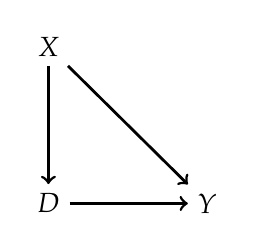
\begin{tikzpicture}
      \node[text centered] (t) {$D$};
      \node[above=1.5 of t, text centered] (x) {$X$};      
      \node[right=1.5 of t, text centered] (y) {$Y$};
      \draw [->, line width= 1] (t) -- (y);
      \draw [->, line width= 1] (x) -- (t);
      \draw [->, line width= 1] (x) -- (y);            
    \end{tikzpicture}
  \end{center}
\end{column}%
\end{columns}
\end{frame}



\begin{frame}{Example of variation necessary in $D$}
\begin{columns}[T] % align columns
\begin{column}{.8\textwidth}
  \begin{wideitemize}
  \item Consider $D$ to be a medical treatment selected by a doctor,
    with $Y$ their subsequent health outcome
    \begin{itemize}
    \item What if $D$ was perfectly predictable by $\mathbf{X}$: e.g., age of
      patient, the doctor's background, etc.
    \item  In other words, if we know $\mathbf{X}$, we know $D$.
    \end{itemize}
  \item Is the effect of $D$ on $Y$ identified, conditional on
    $\mathbf{X}$?
    \pause
  \item No. See this in two ways:
    \begin{itemize}
    \item $Pr(D_{i} | \mathbf{X}_{i})$ = 1 or 0 (fails strong ignorability)       
    \item $Y_{i} = D_{i}\tau + \mathbf{X}_{i}\gamma + \epsilon$ -- perfectly collinear!
    \end{itemize}
  \item Need additional ``exogeneous'' variation
    \end{wideitemize}
\end{column}%
\hfill%
\begin{column}{.4\textwidth}

\end{column}%
\end{columns}
\end{frame}


\begin{frame}{Wanted: exogeneous variation}
\begin{columns}[T] % align columns
\begin{column}{.7\textwidth}
  \begin{wideitemize}
  \item A structural econometrician would describe the variation in
    $D$ as driven by two pieces, $V$ and $X$. Ideally, $V$ is exogeneous.
  \item But what is $V$? Much of the time we don't know.
    \begin{itemize}
    \item This comes back to our research design question -- is there
      something ``near-random'' that caused a difference in treatment? 
    \end{itemize}
  \item More worryingly -- if units are observably identical, but
    choose different outcomes, a purely rational model would suggest
    there are intrinsically different characteristics driving this
    decision. Will this bias our estimates?
    \end{wideitemize}
\end{column}%
\hfill%
\begin{column}{.4\textwidth}

\end{column}%
\end{columns}
\end{frame}




\begin{frame}{Consider a p-score overlap example}
\begin{columns}[T] % align columns
\begin{column}{.5\textwidth}
  \begin{wideitemize}
  \item There are many parts of $\pi(\mathbf{X})$ where there is lots of overlap
  \item In some parts it becomes less common
  \item What does it mean to have so few treated units for the pscore less than 0.5?
    \begin{itemize}
    \item I would worry that these units are somehow not comparable.
    \item If we select away from them, what does that imply about our model estimates?
    \end{itemize}
    \end{wideitemize}
\end{column}%
\hfill%
\begin{column}{.5\textwidth}
\includegraphics[width=\linewidth]{images/overlap1.pdf}
\end{column}%
\end{columns}
\end{frame}



\begin{frame}{Where we will go with this }
  \begin{wideitemize}
  \item A convenient economic model to consider (from Heckman (1997)):
    \begin{align*}
      Y_{i}(0) &= g(X_{i}, D_{i} = 0) + U_{i0}\\
      Y_{i}(1) &= g(X_{i}, D_{i} = 1) + U_{i1}\\
      Y_{i} &= g(X_{i},0) + D_{i}\left(\underbrace{g(X_{i},1) - g(X_{i},0)}_{\text{Average Population Gain}} + \underbrace{U_{i1} - U_{i0}}_{\text{idiosyncratic gain}}\right) + U_{i0}
    \end{align*}
  \item Now we consider what drives the decision making for $D_{i}$:
    \begin{equation*}
      D_{i} = 1( (Y_{i}(1) - Y_{i}(0))   + \kappa + V_{i}  > 0)
    \end{equation*}
    In other words, when the value is sufficiently high (above some
    overall + idiosyncratic cost $\kappa+V_{i}$), I choose to take the program. This creates obvious correlation between $D_{i}$ and $(Y_{i}(0), Y_{i}(1)$
    \end{wideitemize}
\end{frame}


\begin{frame}{Where we will go with this }
    \begin{wideitemize}
    \item Useful to identify when conditioning works:
      \begin{itemize}
      \item Constant effects (e.g. $U_{i1} - U_{i0}$) for everyone
      \item Expectation is the same for everyone ($E(U_{i1} - U_{i0}| X_{i}) = 0$, because of lack of info
      \end{itemize}
    \item The pscore is:
      \begin{equation*}
        Pr(D_{i} = 1 | X_{i}) = Pr\left(g(X_{i},1) - g(X_{i},0) + \kappa + (U_{i1} - U_{i0}) > V_{i} \right) 
      \end{equation*}
    \item Why is this useful? Gives us a framework to consider the economic returns to individuals take a program
    \item What would it take to switch them into the program?
      \begin{enumerate}
      \item Lack of choice -- not always available
      \item Large incentive -- expensive!
      \item High personal returns -- that's good, but selects into a particular type of person
      \end{enumerate}
    \end{wideitemize}
\end{frame}

\begin{frame}{How do we randomly vary people's incentives to move in their pscores?}
\begin{columns}[T] % align columns
\begin{column}{.5\textwidth}
  \begin{wideitemize}
  \item Consider the pscore as an index of valuation
  \item We now want something that varies individuals' valuation
    \begin{itemize}
    \item Will give us ``real'' variation (e.g., avoiding Heckman et al. critique)
    \item Will identify a particular subspace of treated individuals
    \end{itemize}
  \item This is instrumental variables -- a shifter that moves our
    propensity score values in an exogeneous fashion
  \end{wideitemize}
\end{column}%
\hfill%
\begin{column}{.5\textwidth}
\includegraphics[width=\linewidth]{images/overlap3.pdf}
\end{column}%
\end{columns}
\end{frame}


\begin{frame}{How do we randomly vary people's incentives to move in their pscores?}
\begin{columns}[T] % align columns
\begin{column}{.54\textwidth}
  \begin{wideitemize}
  \item Useful to remember this graph when considering how to induce participation
  \item Some folks do not want to participate! 
    \begin{itemize}
    \item Could be perceptions on the returns (e.g. $Y(1) - Y(0)$), rightly or wrongly
    \item \emph{They will be expensive to move}
    \end{itemize}
  \item Your estimand of interest will be considering parts of this distribution
    \begin{itemize}
    \item Useful when considering external validity
    \end{itemize}
  \end{wideitemize}
\end{column}%
\hfill%
\begin{column}{.5\textwidth}
\includegraphics[width=\linewidth]{images/overlap3.pdf}
\end{column}%
\end{columns}
\end{frame}


\end{document}